%\subsection{Automated Fortran kernel generation}\label{sec:kgen}

A significant challenge to optimizing CESM is based on the fact that it is a large and complex application that typically requires expert knowledge to build and execute. Furthermore, it is also resource intensive and requires more then an hour to build and run.  To address these challenges we utilize KGen a python tool that automatically extracts a kernel from large Fortran application \cite{kim2016,kgenrepo}.  This smaller kernel allows pieces of a much larger fortran application to be built and run outside the complexity of the main application.  The KGen generated kernel which is typically from 1K to 30K lines long may take minutes to compile and only seconds to execute, and is easily portable to different compute platforms.  

Working with a kernel, instead of the larger original application has numerous benefits.  These benefits include reducing the time it takes to modify, build, and run code, isolating the impact of code modifications, and  simplify and enhancing collaborations between application developer and compiler and hardware vendors.

KGen has been used extensively in our CESM optimization work.  It has allowed the extraction of a number of kernels for different physical processes including the Morrison Gettelman Microphysics version 2 (MG2) \cite{morrison2015advanced}, the Rapid Radiation Transport Model (RRTMG) \cite{rrtmg}, a Mozart Implicit chemistry solver \cite{mozart}, and the bilinear interpolation. In Section \ref{sec:other} we will describe the optimization of the RRTMG, implicit chemistry solver and the bilinear interpolation code, while the MG2 optimization effort is described in \cite{nesap-web,nesap-paper}.  Most of the KGen kernels are available through a git based repository at \cite{kgenkernels}



%Automatic kernel generation

%Using KGen is a simple one-step process which reduces the amount of time and resource that might be needed if kernel generation is done manually.  Figure 1 shows a workflow of using the tool.

%\begin{figure}[tbp]
% \begin{center}
%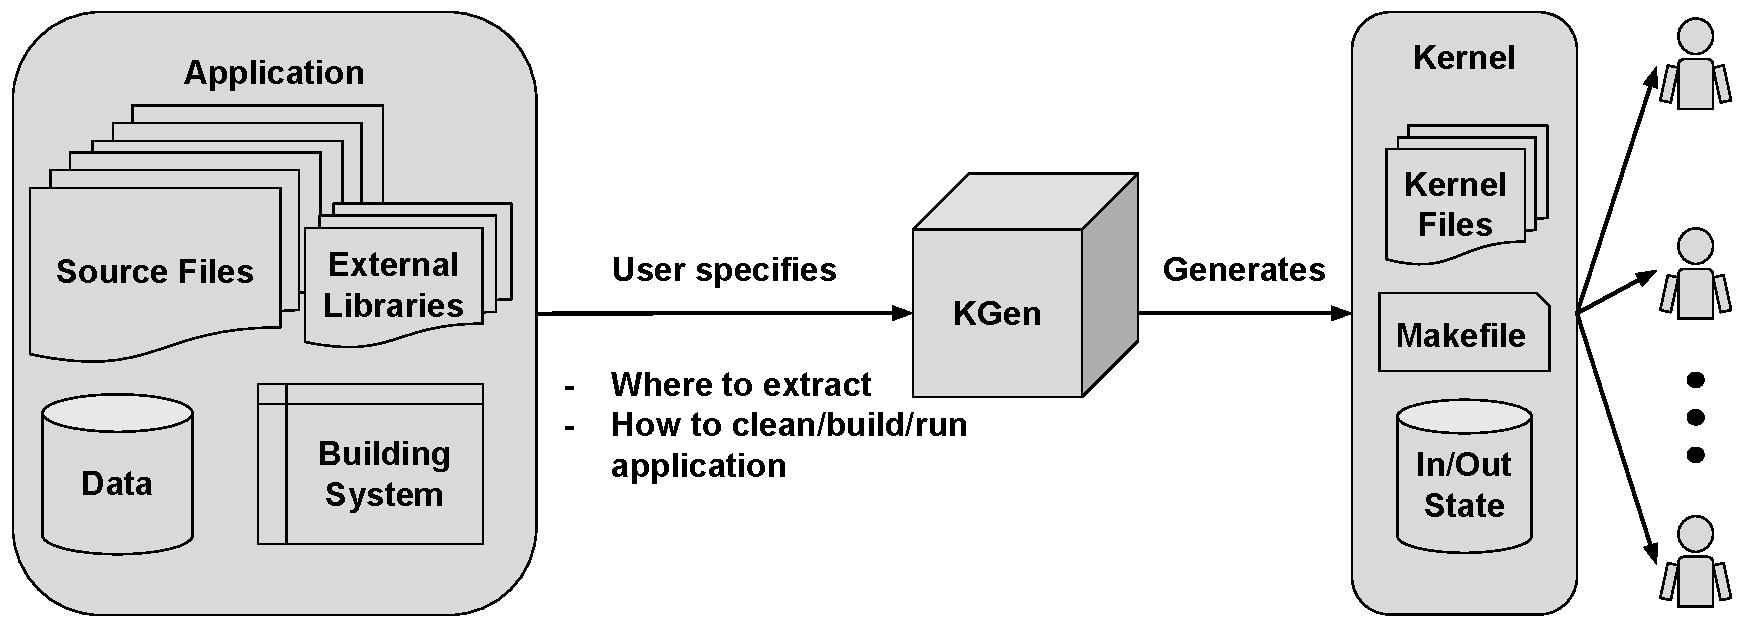
\includegraphics[width=12.0cm]{figures/kgen_workflow.pdf}
%\end{center}
%\caption{KGEN workflow.  {\color{red} Color not allowed in book, excessive space below image.}}
%\label{fig:clmmem}
%\end{figure}



%Since a kernel is a just another software that can be compiled and run independently, its usage is not limited to a particular case. For example, There are several cases that KGen-generated kernel has been used successfully including:

%Performance optimization: Several performance-critical parts of CESM were extracted using KGen and distributed to multiple performance engineers who independently optimized the generated kernels. Optimized kernels are collected and applied to CESM. Validating Float-point calculation among different platforms: The same CESM simulation on two different system showed different simulation result. A �suspicious� part of code was extracted using KGen. After large number of trial-and-errors on the kernel, it is found that the root cause was a FMA(Fused-Multiply-Add) instruction. Compiler bug report: A part of code having a compiler bug is extracted. A compiler bug is reported with the kernel so that the bug could be reproduced easily on compiler vendor site. Porting to GPU: A part of radiation physics code is extracted and shared with an external research team for porting it on GPU. Private benchmark for procurement: One of time consuming part of CESM is extracted and inserted in a benchmark suite for one of recent NCAR procurement.
%A kernel generation example  KGen distribution contains several examples. This section briefly steps through one of the examples to show how to generate a kernel using KGen. First, please make sure that your system meets following prerequisites: Linux OS, Python (higher or equal to 2.7 but less than 3.0), Make build utility, Cpp C preprocessor and Strace system call tracer.

%Downloading KGen: run following Git command on your local directory.
%>>>  git clone  https://github.com/NCAR/KGen.git

%Moving to an example directory: This example shows how to extract a region of Fortran code. Please read README to check if you need any modification for your system setting.
%>>> cd ./KGen/example/simple-region

%Extracting a kernel: run �make� in the example directory. The make command actually invokes KGen command shown below.
%>>>  $KGEN/bin/kgen src/update_mod.F90 --timing repeat=100 \ 
%  --cmd-clean "cd src; make clean" --cmd-build "cd src; make build" --cmd-run "cd src; make run" 
 
%The first argument specifies a path to a source file that contains KGen callsite directives. User can specify any executable region of Fortran code as a kernel region by wrapping the region with �begin_callsite� and �end_callsite� KGen directives. Next �--timing� option is to let KGen run a kernel region 100 times to increase accuracy of timing measurement. The last three options are to let KGen know how to clean/build/run the application. 

%Running a kernel: At this step, kernel files, state data files and Makefile are created in �kernel� subdirectory. Running KGen-generated Makefile in �kernel� directory will build/run the kernel and shows the results of verification and timing measurement of the kernel.
%>>> cd kernel; make


